\documentclass[12pt]{article}
\usepackage{amsmath}
\newcommand{\myvec}[1]{\ensuremath{\begin{pmatrix}#1\end{pmatrix}}}
\newcommand{\mydet}[1]{\ensuremath{\begin{vmatrix}#1\end{vmatrix}}}
\newcommand{\solution}{\noindent \textbf{Solution: }}
\providecommand{\brak}[1]{\ensuremath{\left(#1\right)}}
\providecommand{\norm}[1]{\left\lVert#1\right\rVert}
\let\vec\mathbf
\usepackage{graphicx}
\usepackage{float}

\title{Coordinate Geometry}
\author{SAMEERGUPTA(sameergupta@sriprakashschools.com)}
\begin{document}
\maketitle
\section*{10$^{th}$ Maths - Chapter 7}
This is Problem-1.2 from Exercise 7.1
\begin{enumerate}
\item Find the distance between the following pairs of points.\\
 ii)(– 5, 7),(– 1, 3).\\
\solution:\\
Given,
\begin{align}
\vec{A}&=\myvec{-5\\7}\\
\vec{B}&=\myvec{-1\\3}\\
\vec{AB}&=\myvec{4\\-4}\\
\norm{AB}&=\sqrt{(4)^2+(-4)^2}\\
\norm{AB}&=\sqrt{16+16}\\
\norm{AB}&=\sqrt{32}\\
\norm{AB}&=2\sqrt{4}\\
\end{align}
\end{enumerate}
\begin{figure}[H]
			\centering
			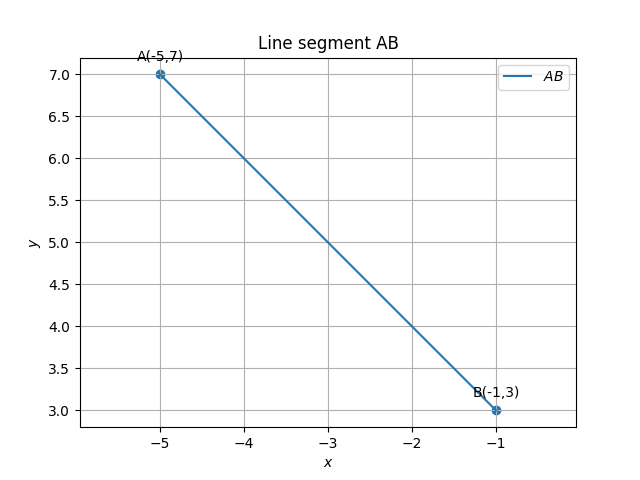
\includegraphics[width=\columnwidth]{figs/Figure_1.png}
			\caption{Line segment AB}
			\label{fig:13}
		\end{figure}

\end{document}
